\chapter{آبار الكمون والحواجز والنفق}\label{ch:b2:potential-wells-tunneling}

الكرة في وعاء تتدحرج جيئةً وذهابًا بأي طاقة أُعطيت
إياها؛ أما الإلكترون في ذرة، والنوية في نواة، والإلكترون في
بلورة بحجم النانومتر فلا يمكن أن تكون لها إلا طاقات معينة، وأدناها
ليس صفرًا. والكرة لا تستطيع عبور تلّ أعلى مما تسمح به طاقتها؛
أما جسيم $\alpha$ فيغادر نواة عبر جدار كولوني
ما كان ليتسلقه أبدًا، وإبرة مجهر النفق الماسح تسحب
تيارًا عبر فجوة من الخلاء، وذرة الآزوت في النشادر
تتأرجح عبر مستوي هدروجيناتها الثلاثة أربعًا وعشرين مليار
مرة في الثانية. وهذا الفصل يحلّ معادلة شرودنغر في
أبسط الكمونات --- آبار بجدران لانهائية ومنتهية، ودرجة، و
حاجز، وبئر مزدوجة --- ويجد فيها الواقعتين الكموميتين الكبيرتين
اللتين لا يستطيع الميكانيك الكلاسيكي إنتاجهما: \emph{تكميم}
الطاقات المرتبطة، و\emph{النفق} عبر المناطق الممنوعة كلاسيكيًّا،
مع حساسيته الأسّية لعرض الحاجز وارتفاعه، ولهذا يصلح
مسطرةً للبيكومترات ولهذا تمتد أعمار النشاط الإشعاعي على
ثلاثين رتبة من المقدار.

\begin{omfigure}
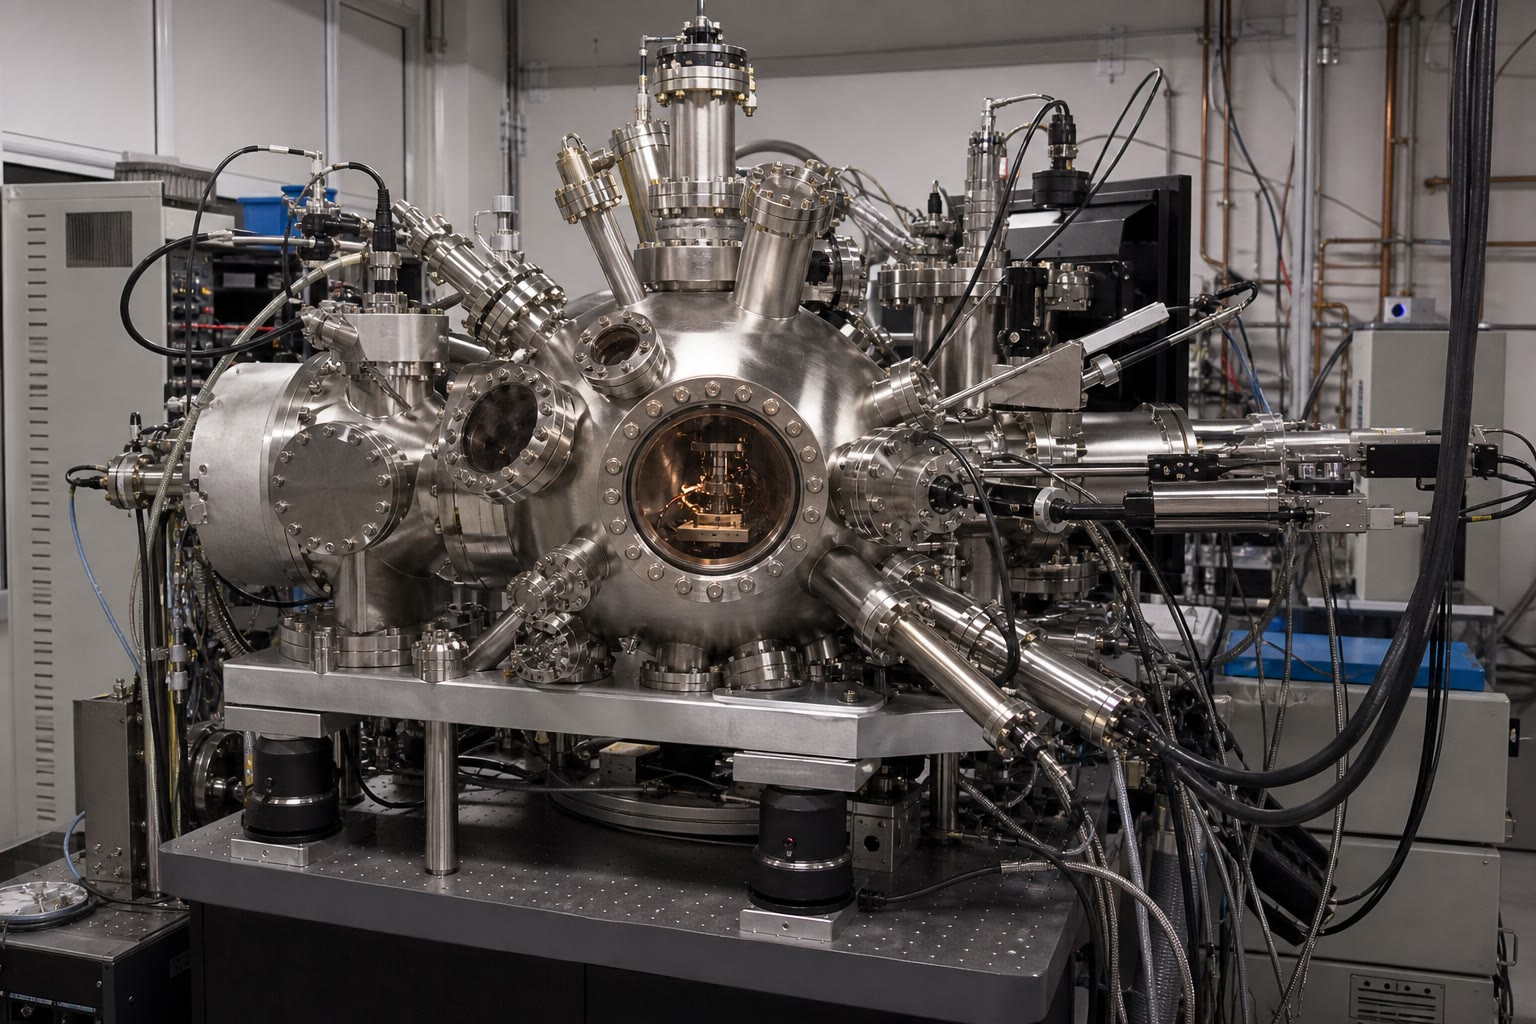
\includegraphics[width=0.58\linewidth]{images/book4/ai/b4-31-stm-instrument.jpg}

{\small مجهر نفق ماسح: طرف معدني يُمسَك على بضعة
أعشار النانومتر فوق سطح؛ وتيار النفق، الذي
يتغير بعشرة أضعاف في كل عُشر نانومتر، يرسم السطح ذرةً
ذرة.}
\end{omfigure}

\section{البئر اللانهائية}

\begin{proposition}[البئر المربعة اللانهائية]\label{prop:b2:potential-wells-tunneling:infinite}
جسيم محبوس في $0 < x < L$ بجدران لا تُخترَق ($V = 0$
في الداخل، و $V = \infty$ في الخارج، ومن ثَمّ $\varphi = 0$ عند الجدارين) له
\omterm{thm:b2:schrodinger-wave-functions:stationary}{الحالات المستقرة} والطاقات
\[
\varphi_n(x) = \sqrt{\frac{2}{L}}\sin\frac{n\pi x}{L}, \qquad
E_n = \frac{n^2h^2}{8mL^2} = n^2E_1, \qquad n = 1, 2, 3, \dots
\]
فالطاقات \emph{مكمَّمة}\index{تكميم الطاقة}، وتنمو
وفق $n^2$، وأدناها ليس صفرًا: و\emph{طاقة
الحبس}\index{طاقة الحبس} $E_1 = h^2/8mL^2$ هي ثمن
التوضيع (إذ يفرض $\Delta x \sim L$ أن $\Delta p \sim h/2L$). والتوابع
$\varphi_n$ متعامدة، $\int\varphi_n\varphi_m\dd x = \delta_{nm}$، وكل
حالة في البئر تراكب لها.
\end{proposition}

\begin{proof}
في الداخل، $\varphi'' = -k^2\varphi$ مع $k^2 = 2mE/\hbar^2$: $\varphi = A\sin kx
+ B\cos kx$؛ و $\varphi(0) = 0$ يلغي $B$، و $\varphi(L) = 0$ يقتضي $kL = n\pi$
--- أي الأمواج المستقرة على وتر، مع $E = \hbar^2k^2/2m$.
والتنظيم يعطي $A = \sqrt{2/L}$؛ والتعامد هو تعامد
الجيوب.
\end{proof}

\begin{omfigure}
\begin{tikzpicture}[scale=0.9]
  \draw[thick] (0,0) -- (0,4.6); \draw[thick] (4,0) -- (4,4.6); \draw[thick] (0,0) -- (4,0);
  \foreach \n/\y/\c in {1/0.45/omDef, 2/1.8/omThm, 3/4.05/omExo}{
    \draw[\c, thick] (0,\y) -- (4,\y);
    \node[font=\scriptsize, \c, right] at (4.1,\y) {$E_\n = \n^2E_1$};
    \draw[\c, thick, domain=0:4, samples=80] plot (\x,{\y+0.35*sin(deg(\n*pi*\x/4))});
  }
  \node[font=\scriptsize] at (2,-0.35) {$0 < x < L$};
  \begin{scope}[xshift=7.5cm]
    \draw[thick] (0,0) -- (0,4.6); \draw[thick] (4,0) -- (4,4.6); \draw[thick] (0,0) -- (4,0);
    \foreach \n/\y/\c in {1/0.45/omDef, 2/1.8/omThm, 3/4.05/omExo}{
      \draw[\c, thick, domain=0:4, samples=80] plot (\x,{\y+0.5*(sin(deg(\n*pi*\x/4)))^2});
      \draw[gray!60, thin] (0,\y) -- (4,\y);
    }
    \node[font=\scriptsize] at (2,-0.35) {$|\varphi_n|^2$};
  \end{scope}
\end{tikzpicture}

{\small البئر اللانهائية: أول ثلاثة مستويات، $E_n \propto n^2$،
مع توابعها الموجية (على اليسار) وكثافات احتمالها (على اليمين) ---
أي $n - 1$ عقدة، وحالة أساسية منتشرة في البئر
ولها طاقة غير معدومة.}
\end{omfigure}

\begin{example}[رتب المقادير، والألوان]\label{ex:b2:potential-wells-tunneling:orders}
$E_1 = h^2/8mL^2$: فلإلكترون في \qty{1}{nm}، \qty{0.38}{eV}؛ وفي
\qty{0.1}{nm} (أي ذرة)، \qty{38}{eV} --- وهو سلّم الطاقات الذرية؛ ولنوية
في \qty{5}{fm}، \qty{8}{MeV} --- وهو سلّم الطاقات النووية؛ ولكرة
زجاجية في صندوق، $10^{-63}\,\unit{J}$ --- فلن يلاحظ أحد. وبلورة
نانوية نصف ناقلة عرضها بضعة نانومترات (أي \emph{نقطة
كمومية}) تحبس إلكتروناتها: فتضاف \omterm{prop:b2:potential-wells-tunneling:infinite}{طاقة الحبس} إلى
فجوة البلورة، وكلما صغرت النقطة ازرقّ ضوءها ---
فالمادة نفسها تتوهج حمراء عند \qty{6}{nm} وخضراء عند \qty{3}{nm}،
مضبوطةً بالحجم وحده.
\end{example}

\section{البئر المنتهية}

\begin{proposition}[البئر المربعة المنتهية]\label{prop:b2:potential-wells-tunneling:finite}
من أجل $V = 0$ في $|x| < a$ و $V = V_0$ في الخارج، تتذبذب حالة $0 < E < V_0$
في الداخل ($k = \sqrt{2mE}/\hbar$) وتتخامد في الخارج ($\kappa =
\sqrt{2m(V_0 - E)}/\hbar$): $\varphi \propto \eu^{-\kappa|x|}$ وراء الجدارين.
وموافقة $\varphi$ و $\varphi'$ عند $x = \pm a$ تعطي، من أجل الحالتين الزوجية والفردية،
\[
k\tan ka = \kappa \quad\text{(زوجي)}, \qquad
-k\cot ka = \kappa \quad\text{(فردي)}, \qquad\text{مع}\quad
(ka)^2 + (\kappa a)^2 = \frac{2mV_0a^2}{\hbar^2} \equiv R^2 .
\]
وهندسيًّا، تكون الحلول تقاطعات المنحنيين $\eta =
\xi\tan\xi$ و $\eta = -\xi\cot\xi$ مع الدائرة $\xi^2 + \eta^2 = R^2$
($\xi = ka$، و $\eta = \kappa a$): فثمة \emph{دائمًا حالة مرتبطة واحدة
على الأقل} (وهي الحالة الأساسية الزوجية)، و $1 + \lfloor 2R/\pi\rfloor$ في الكلّ.
والجسيم \emph{ينفذ} في المنطقة الممنوعة على العمق
$1/\kappa$، وتقع المستويات دون مستويات البئر اللانهائية ذات
العرض نفسه.
\end{proposition}

\begin{proof}
الحلّ الزوجي هو $A\cos kx$ في الداخل و $B\eu^{-\kappa|x|}$ في الخارج؛ و
استمرار $\varphi'/\varphi$ عند $x = a$ يعطي $-k\tan ka = -\kappa$. والأمر
نفسه من أجل الفردي مع $\sin$. والدائرة هي تعريف $k$ و
$\kappa$. وكل فرع من $\xi\tan\xi$ يبدأ عند $\xi = n\pi$ ومن
$-\xi\cot\xi$ يبدأ عند $(n + \tfrac12)\pi$ يلاقي الدائرة مرة إن
بدأ داخلها: ومن هنا العدّ.
\end{proof}

\begin{omfigure}
\begin{tikzpicture}
  \begin{axis}[omaxis, width=8.6cm, height=5cm, xmin=0, xmax=5.2, ymin=0, ymax=5.2,
    xlabel={$\xi = ka$}, ylabel={$\eta = \kappa a$}, xtick={1.571,3.142,4.712}, xticklabels={$\pi/2$,$\pi$,$3\pi/2$}, ytick=\empty, clip=true,
    legend style={font=\scriptsize, at={(0.98,0.98)}, anchor=north east, draw=none, fill=white}]
    \addplot[omDef, thick, domain=0:1.5, samples=80] {x*tan(deg(x))};
    \addlegendentry{$\xi\tan\xi$ (زوجي)}
    \addplot[omExo, thick, domain=1.6:3.1, samples=80] {-x/tan(deg(x))};
    \addlegendentry{$-\xi\cot\xi$ (فردي)}
    \addplot[omDef, thick, domain=3.2:4.65, samples=80] {x*tan(deg(x))};
    \addplot[omExo, thick, domain=4.75:5.2, samples=40] {-x/tan(deg(x))};
    \addplot[omThm, thick, domain=0:4, samples=100] {sqrt(16-x*x)};
    \addlegendentry{$\xi^2 + \eta^2 = R^2$}
    \addplot[gray, dashed, domain=0:1.2, samples=40] {sqrt(1.44-x*x)};
  \end{axis}
\end{tikzpicture}

{\small الحلّ الهندسي للبئر المنتهية: الحالات المرتبطة هي
تقاطعات الدائرة التي نصف قطرها $R = a\sqrt{2mV_0}/\hbar$ مع
الفرعين $\xi\tan\xi$ (الحالات الزوجية) و $-\xi\cot\xi$ (الفردية). وهنا
$R = 4$: أي ثلاث حالات مرتبطة؛ والدائرة الصغيرة المتقطعة ($R = 1.2$) لا تزال
تقطع الفرع الأول --- فالبئر تربط دائمًا حالة واحدة على الأقل.}
\end{omfigure}

\begin{example}[إلكترون في بئر بالنانومتر]\label{ex:b2:potential-wells-tunneling:finite}
$V_0 = \qty{1}{eV}$، والعرض $2a = \qty{1}{nm}$: $R = a\sqrt{2mV_0}/\hbar = 0.5 \times
10^{-9} \times 5.1 \times 10^9 = 2.6$، ومن ثَمّ $1 + \lfloor 2R/\pi\rfloor = 2$ حالة
مرتبطة؛ وتقع الحالة الأساسية قرب \qty{0.26}{eV} بدل \qty{0.38}{eV}
في البئر اللانهائية، وتتسرب \qty{0.2}{nm} في الجدارين
($1/\kappa = \hbar/\sqrt{2m(V_0 - E)}$). وآبار كهذه، تُنمَّى طبقاتٍ من
أنصاف النواقل بسماكة بضعة نانومترات، هي قلب
ثنائيات الليزر في \cref{ch:b2:laser}.
\end{example}

\section{الدرجة والحاجز: النفق}

\begin{proposition}[درجة كمون]\label{prop:b2:potential-wells-tunneling:step}
جسيم طاقته $E$ قادم من $x < 0$ على الدرجة $V = V_0$
من أجل $x > 0$:
\begin{itemize}
\item $E > V_0$: $\varphi = \eu^{\iu k_1x} + r\eu^{-\iu k_1x}$ على اليسار، و $t\eu^{\iu
      k_2x}$ على اليمين، مع $k_{1,2} = \sqrt{2m(E - V_{0,\text{يسار/يمين}})}/
      \hbar$؛ واستمرار $\varphi$ و $\varphi'$ يعطي $r = (k_1 - k_2)/(k_1
      + k_2)$ واحتمال الانعكاس (وهو نسبة التيارين) $R = r^2$،
      و $T = 1 - R = 4k_1k_2/(k_1 + k_2)^2$ --- فالجسيم \emph{يمكن أن
      ينعكس على درجة له من الطاقة ما يتسلقها}، تمامًا كموجة على
      وتر عند تغيّر ممانعة (\cref{ch:b2:wave-interfaces})؛
\item $E < V_0$: وعلى اليمين $\varphi = t\eu^{-\kappa x}$، مع $\kappa = \sqrt{2m(V_0
      - E)}/\hbar$ --- أي \emph{موجة متلاشية}\index{موجة متلاشية
      (كمومية)}؛ و $|r| = 1$ (أي انعكاس كلي، مع انزياح طور)، ولا
      يجري تيار إلى الدرجة، لكن الجسيم يوجد هناك باحتمال
      يتخامد على $1/\kappa$.
\end{itemize}
\end{proposition}

\begin{proof}
اكتب معادلات الاستمرار عند $x = 0$ وحلّها؛ ومن أجل التيارات
استعمل $j = (|A|^2 - |B|^2)\hbar k/m$ (\cref{ch:b2:schrodinger-wave-functions}).
ومن أجل $E < V_0$، $r = (k - \iu\kappa)/(k + \iu\kappa)$، وطويلته واحد.
\end{proof}

\begin{theorem}[النفق عبر حاجز]\label{thm:b2:potential-wells-tunneling:tunnel}
جسيم طاقته $E < V_0$ يلاقي حاجزًا مستطيلًا ارتفاعه
$V_0$ وعرضه $a$ ينفذ باحتمال
\[
T = \Big[1 + \frac{V_0^2\sinh^2(\kappa a)}{4E(V_0 - E)}\Big]^{-1}
\ \approx\ 16\,\frac{E}{V_0}\Big(1 - \frac{E}{V_0}\Big)\eu^{-2\kappa a}
\quad (\kappa a \gg 1), \qquad
\kappa = \frac{\sqrt{2m(V_0 - E)}}{\hbar} .
\]
وهذا هو \emph{أثر النفق}\index{أثر النفق}: وهو مستحيل
كلاسيكيًّا، وصغير أسّيًّا في الميكانيك الكمومي --- وحساس
أسّيًّا للعرض $a$ وللارتفاع $V_0 - E$ وللكتلة
$m$. فمن أجل إلكترون \qty{1}{eV} دون القمة، $\kappa = \qty{5.1}{nm^{-1}}$:
$T \sim 10^{-2}$ من أجل $a = \qty{0.5}{nm}$، و $10^{-4}$ من أجل \qty{1}{nm}، و $10^{-9}$ من أجل
\qty{2}{nm}؛ وأما البروتون فيكون $\kappa$ له أكبر $43$ مرة ولا ينفذ شيء
عند هذه العروض.
\end{theorem}

\begin{proof}
$\varphi = \eu^{\iu kx} + r\eu^{-\iu kx}$ من أجل $x < 0$، و $A\eu^{\kappa x} + B\eu^{-\kappa x}$
في الداخل، و $t\eu^{\iu kx}$ من أجل $x > a$؛ وأربعة شروط استمرار (على $\varphi$
و $\varphi'$ عند $0$ و $a$) من أجل أربعة مجاهيل؛ وبإزالة $A$ و $B$ و $r$
نحصل على $1/|t|^2 = 1 + (k^2 + \kappa^2)^2\sinh^2(\kappa a)/4k^2\kappa^2$، وهي
الصيغة مع $k^2 = 2mE/\hbar^2$ و $\kappa^2 = 2m(V_0 - E)/\hbar^2$. ومن أجل
$\kappa a \gg 1$، $\sinh\kappa a \approx \eu^{\kappa a}/2$. ومن أجل حاجز
اعتباطي الشكل يصير الأسّ $2\int\kappa(x)\dd x$ عبر
المنطقة الممنوعة (وهو عامل غاموف، مقبول).
\end{proof}

\begin{omfigure}
\begin{tikzpicture}[scale=0.9, >=stealth]
  \fill[gray!15] (3,0) rectangle (4.2,2.6);
  \draw[thick] (0,0) -- (3,0) -- (3,2.6) -- (4.2,2.6) -- (4.2,0) -- (7.5,0);
  \draw[dashed, omExo] (0,1.2) -- (7.5,1.2) node[right, font=\scriptsize] {$E$};
  \node[font=\scriptsize] at (3.6,2.85) {$V_0$};
  \draw[<->, thin] (3,-0.3) -- (4.2,-0.3) node[midway, below, font=\scriptsize] {$a$};
  % الموجة: واردة ومنعكسة (يسارًا)، ومتلاشية (داخلًا)، ونافذة (يمينًا)
  % wave: incident+reflected (left), evanescent (inside), transmitted (right)
  \draw[omDef, thick, domain=0:3, samples=120] plot (\x,{1.2+0.5*cos(deg(6*\x))});
  \draw[omDef, thick, domain=3:4.2, samples=40] plot (\x,{1.2+0.5*exp(-1.6*(\x-3))});
  \draw[omDef, thick, domain=4.2:7.5, samples=120] plot (\x,{1.2+0.073*cos(deg(6*(\x-4.2)))});
  \node[font=\scriptsize, omDef] at (1.5,2.1) {$\eu^{\iu kx} + r\eu^{-\iu kx}$};
  \node[font=\scriptsize, omDef] at (3.6,1.95) {$\eu^{-\kappa x}$};
  \node[font=\scriptsize, omDef] at (6.0,1.75) {$t\eu^{\iu kx}$, $|t|^2 \approx 16\frac{E}{V_0}(1 - \frac{E}{V_0})\eu^{-2\kappa a}$};
\end{tikzpicture}

{\small النفق عبر حاجز: تتذبذب الموجة على اليسار، و
تتخامد أسّيًّا داخل المنطقة الممنوعة كلاسيكيًّا، و
تخرج على اليمين بسعة منخفضة --- بطول الموجة نفسه،
وباحتمال صغير.}
\end{omfigure}

\begin{example}[مجهر النفق الماسح]\label{ex:b2:potential-wells-tunneling:stm}
يُقرَّب طرف معدني حادّ إلى $d \approx \qty{0.5}{nm}$ من
سطح ناقل ويُطبَّق توتر صغير: فتنفق الإلكترونات عبر
فجوة الخلاء، وارتفاع حاجزها هو تابع العمل $\Phi \approx
\qty{4.5}{eV}$، ومن ثَمّ $\kappa = \sqrt{2m\Phi}/\hbar = \qty{1.1e10}{m^{-1}}$ و
يتغير التيار $I \propto \eu^{-2\kappa d}$ بالعامل $\eu^{2.2} \approx
10$ في كل \qty{0.1}{nm}. وحلقة \omterm{def:b2:feedback-oscillators:loop}{تغذية راجعة} تحرّك الطرف لتبقي $I$
ثابتًا، وارتفاع الطرف، مسجَّلًا وهو يمسح، يرسم السطح
بتمييز شاقولي قدره بيكومتر --- وعرضًا ذرةً
ذرة، لأن آخر ذرة في الطرف، وهي الأقرب، تحمل معظم
التيار (بينيغ وروهرر، 1981).
\end{example}

\begin{example}[التفكك ألفا]\label{ex:b2:potential-wells-tunneling:alpha}
جسيم $\alpha$ طاقته \qty{5}{MeV} داخل نواة ثقيلة يواجه
حاجز كولون للشحنة الباقية $Ze$، وارتفاعه عشرات الميغا إلكترون فولت عند
سطح النواة ويمتد إلى نصف القطر $b = 2Ze^2/4\pi\varepsilon_0E
\approx \qty{50}{fm}$ حيث $V = E$. وعامل غاموف $2\int\kappa\,\dd r$
من رتبة $80$: $T \sim \eu^{-80} \sim 10^{-35}$. والجسيم يصدم الجدار
نحو $10^{21}$ مرة في الثانية، فيفلت بمعدل $\sim 10^{-14}
\,\unit{s^{-1}}$: أي عمر قدره مليون سنة. ولأن الأسّ
يتغير وفق $Z/\sqrt E$، فإن تغيّرًا قدره $\qty{2}{MeV}$ في $E$ يزيح العمر
بعشرين رتبة من المقدار --- وهو قانون غايغر--نوتال، من
الميكروثواني إلى عمر الكون (غاموف، 1928: وهو أول
تطبيق للنفق).
\end{example}

\begin{omfigure}
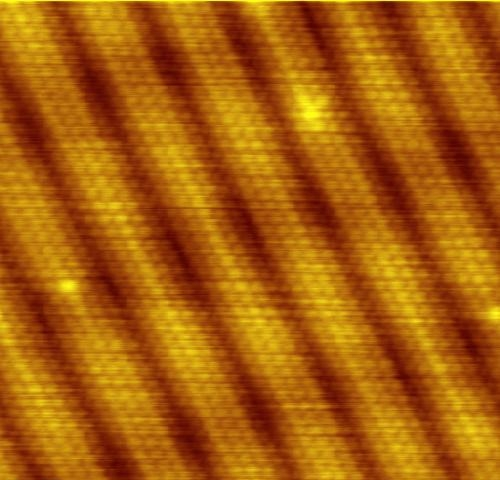
\includegraphics[width=0.42\linewidth]{images/book4/stm-gold-100.jpg}

{\small تمييز ذري على سطح ذهب، مصوَّرًا بمجهر نفق ماسح: صفوف ذرات الوجه (100) المعاد بناؤه، متباعدة بضعة أعشار النانومتر.}
\end{omfigure}

\section{البئر المزدوجة}

\begin{proposition}[انشقاق النفق]\label{prop:b2:potential-wells-tunneling:double}
بئران متطابقتان يفصلهما حاجز: فلو كان الحاجز
لا يُخترَق لكان لكل بئر المستوي الأساسي نفسه $E_0$، مرتين.
والنفق يقرنهما فتكون أدنى حالتي البئر المزدوجة
هما التركيبين \emph{المتناظر} و\emph{اللامتناظر}،
$\varphi_\pm \approx (\varphi_{\text{يسار}} \pm \varphi_{\text{يمين}})/\sqrt2$، وطاقتاهما
$E_0 \mp \Delta/2$: فينشقّ المستوي \emph{انشقاقًا} مقداره $\Delta \propto
\eu^{-\kappa a}$ (وهي سعة النفق، لا مربعها). والجسيم
الموضوع في البئر اليسرى، $\psi = (\varphi_+ + \varphi_-)/\sqrt2$، ليس
مستقرًّا: بل يتذبذب بين البئرين بالتواتر
$\nu = \Delta/h$ --- وهي \emph{تذبذبات النفق}، أي ضربات المستويين في
\cref{ch:b2:schrodinger-wave-functions}.
\end{proposition}

\begin{proof}
التركيب المتناظر لا عقدة له تحت الحاجز وتقوّسه
أدنى، ومن ثَمّ طاقته أدنى؛ واللامتناظر له عقدة و
يقع أعلى؛ والانشقاق متناسب مع تراكب التوابع
الموضَّعة تحت الحاجز، $\eu^{-\kappa a}$. والضربات هي
تراكب المستويين المحسوب أصلًا.
\end{proof}

\begin{omfigure}
\begin{tikzpicture}[scale=0.9]
  % كمون البئر المزدوجة
  \draw[thick] (0,3) -- (0,0) -- (1.8,0) -- (1.8,1.6) -- (2.4,1.6) -- (2.4,0) -- (4.2,0) -- (4.2,3);
  \draw[omDef, thick] (0,0.7) -- (4.2,0.7); \node[font=\scriptsize, omDef, right] at (4.3,0.62) {$E_0 - \Delta/2$};
  \draw[omExo, thick] (0,1.0) -- (4.2,1.0); \node[font=\scriptsize, omExo, right] at (4.3,1.08) {$E_0 + \Delta/2$};
  \begin{scope}[xshift=7.2cm]
    \draw[thick] (0,3) -- (0,0) -- (1.8,0) -- (1.8,1.6) -- (2.4,1.6) -- (2.4,0) -- (4.2,0) -- (4.2,3);
    \draw[omDef, thick, domain=0:1.8, samples=50] plot (\x,{2.2+0.5*sin(deg(pi*\x/1.8))});
    \draw[omDef, thick] (1.8,2.2) .. controls (2.0,2.27) and (2.2,2.27) .. (2.4,2.2);
    \draw[omDef, thick, domain=2.4:4.2, samples=50] plot (\x,{2.2+0.5*sin(deg(pi*(\x-2.4)/1.8))});
    \node[font=\scriptsize, omDef, right] at (4.3,2.3) {$\varphi_+$ متناظر};
    \draw[omExo, thick, domain=0:1.8, samples=50] plot (\x,{0.9+0.5*sin(deg(pi*\x/1.8))});
    \draw[omExo, thick] (1.8,0.9) .. controls (2.0,0.83) and (2.2,0.97) .. (2.4,0.9);
    \draw[omExo, thick, domain=2.4:4.2, samples=50] plot (\x,{0.9-0.5*sin(deg(pi*(\x-2.4)/1.8))});
    \node[font=\scriptsize, omExo, right] at (4.3,0.9) {$\varphi_-$ لامتناظر};
  \end{scope}
\end{tikzpicture}

{\small البئر المزدوجة: المستوي المنحلّ في البئرين المعزولتين
ينشقّ إلى حالة متناظرة (أدنى) وأخرى لامتناظرة
(أعلى) بمقدار $\Delta \propto \eu^{-\kappa a}$؛ والجسيم المبدوء به على جهة
ينفق جيئةً وذهابًا بالتواتر $\Delta/h$.}
\end{omfigure}

\begin{example}[النشادر]\label{ex:b2:potential-wells-tunneling:ammonia}
في NH$_3$ تقع ذرة الآزوت على جهة من مستوي الهدروجينات
الثلاثة أو على الأخرى --- أي بئر مزدوجة بحاجز نحو
\qty{0.25}{eV}. وانشقاق نفق المستوي الأساسي هو $\Delta =
\qty{1e-4}{eV}$: $\nu = \Delta/h = \qty{24}{GHz}$، وهو تواتر
\emph{القلب}، وهو انتقال أول ميزر وأول ساعة
ذرية (1949). واستبدل بالهدروجين الديوتيريوم فينفق الجزيء الأثقل
أقلّ: \qty{1.6}{GHz}. وفي الأهرام الأثقل (PH$_3$ و أرسين) ينهار
الانشقاق إلى الكيلوهرتزات وما دونها: فيبقى الجزيء على
جهته سنين --- ولهذا توجد الجزيئات اليسراوية واليمناوية
أصلًا، ولهذا لا يترصّع السكر على الرفّ.
\end{example}

\begin{omfigure}
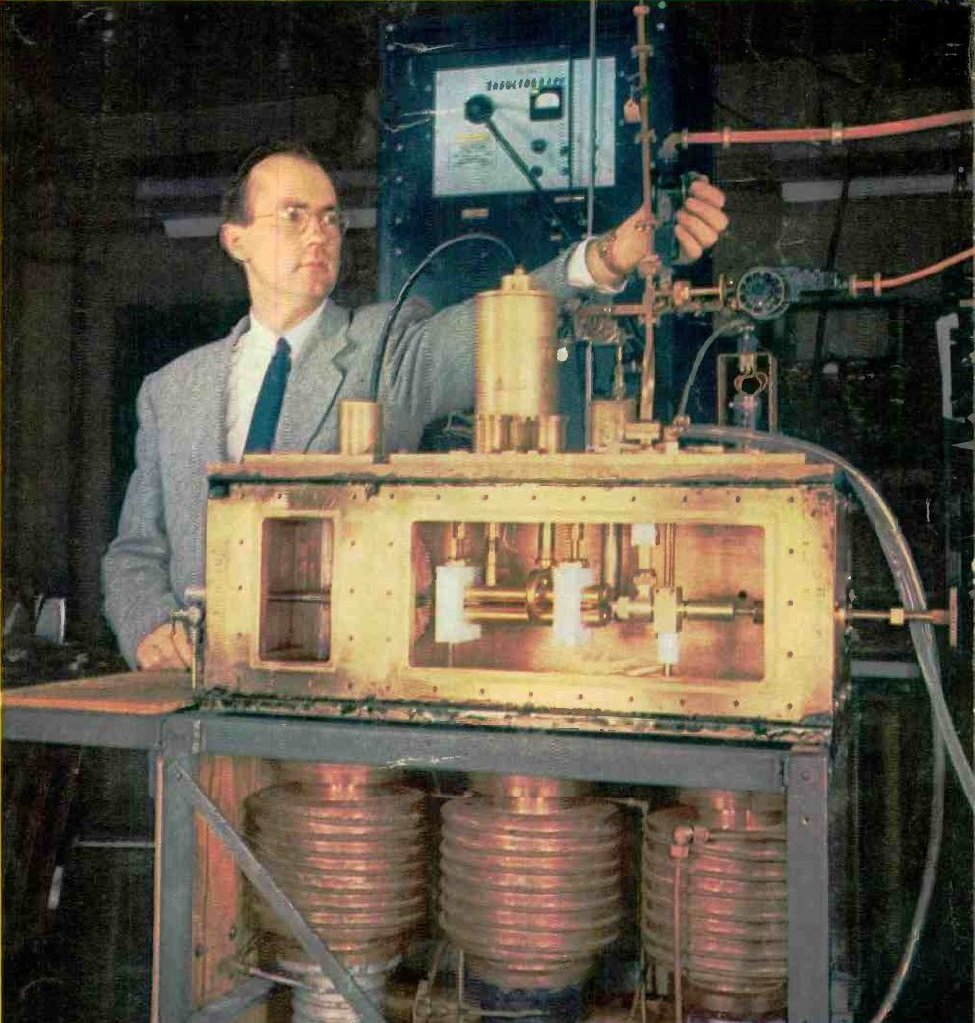
\includegraphics[width=0.5\linewidth]{images/book4/townes-maser.jpg}

{\small تشارلز تاونز مع أول ميزر (1954): حزمة من جزيئات النشادر، مفروزة بحقل كهربائي إلى حالة القلب العليا، ضخّمت انتقال \qty{24}{GHz} في جوف --- وهو أول جهاز \omterm{def:b2:laser:processes}{للإصدار المستحثّ}، قبل الليزر بستّ سنين.}
\end{omfigure}

\begin{method}[الآبار والحواجز]\label{meth:b2:potential-wells-tunneling:method}
(1) اكتب $\varphi$ منطقةً منطقة: $\eu^{\pm\iu kx}$ حيث $E > V$،
و $\eu^{\pm\kappa x}$ حيث $E < V$، مع $k, \kappa = \sqrt{2m|E - V|}/\hbar$.
(2) ووافق $\varphi$ و $\varphi'$ عند كل حدّ (وعند جدار لانهائي،
$\varphi = 0$). (3) وأما الحالات المرتبطة: فللموافقة حلول من أجل
$E$ منفصلة لا غير --- فعُدّها هندسيًّا. (4) وأما التبعثر: فالتيارات
$(|A|^2 - |B|^2)\hbar k/m$ تعطي $R$ و $T$. (5) وأما النفق: فيكون $T \sim
\eu^{-2\kappa a}$؛ ورتبة المقدار أولًا، والعامل بعد ذلك. (6)
والبئر المزدوجة: الانشقاق $\propto\eu^{-\kappa a}$، والضربات عند $\Delta/h$.
\end{method}

\section{تمارين}

\begin{exercise}[$\star$]\label{exo:b2:potential-wells-tunneling:1}
البئر اللانهائية: إلكترون في \qty{1}{nm} (أوجد $E_1$، و $E_2$، و $E_3$، وطول موجة
فوتون $2 \to 1$)؛ وإلكترون في \qty{0.1}{nm}؛ ونوية في \qty{5}{fm}؛
وكرة زجاجية \qty{1}{g} في \qty{10}{cm} ($E_1$، والعدد الكمومي من أجل
سرعة \qty{1}{cm/s}).
\end{exercise}

\begin{exercise}[$\star$]\label{exo:b2:potential-wells-tunneling:2}
النقاط الكمومية: بلورة نانوية فجوتها \qty{1.74}{eV} تحبس زوج
إلكترون وثقب طاقة حبسه $h^2/8m^*L^2$ مع
$m^* = 0.1\,m_{\text{e}}$. أوجد طول موجة الإصدار من أجل $L = 6$، و $4$، و $3$،
و \qty{2.5}{nm}؛ وأي الألوان؟
\end{exercise}

\begin{exercise}[$\star$]\label{exo:b2:potential-wells-tunneling:3}
النفق: إلكترون مع $V_0 - E = \qty{4.5}{eV}$: أوجد $\kappa$؛ و $\eu^{-2\kappa a}$
من أجل $a = 0.3$، و $0.5$، و $1$، و \qty{2}{nm}؛ والعامل في كل \qty{0.1}{nm}؛ وأعد ذلك من أجل
بروتون عند $a = \qty{0.3}{nm}$.
\end{exercise}

\begin{exercise}[$\star$]\label{exo:b2:potential-wells-tunneling:4}
الدرجة: إلكترون \qty{2}{eV} على درجة \qty{1}{eV}: أوجد $k_1$، و $k_2$،
و $R$، و $T$. وأعد ذلك من أجل درجة نازلة \qty{1}{eV}. ولمَ يكون ذلك مستحيلًا
كلاسيكيًّا، وما نظيره في الضوء؟
\end{exercise}

\begin{exercise}[$\star\star$]\label{exo:b2:potential-wells-tunneling:5}
\emph{البئر اللانهائية بالتفصيل.} (أ) استنتج المستويات ونظِّم.
(ب) وبيّن التعامد. (ج) ومن أجل $n = 1$: أوجد $\langle x\rangle$، و $\Delta x =
L\sqrt{1/12 - 1/2\pi^2}$، و $\langle p\rangle = 0$، و $\Delta p = \pi\hbar/L$؛ وتحقق من
هايزنبرغ. (د) وارسم $|\varphi_n|^2$ من أجل $n$ الكبيرة وقارنه بالاحتمال
الكلاسيكي لإيجاد جسيم يرتدّ.
\end{exercise}

\begin{exercise}[$\star\star$]\label{exo:b2:potential-wells-tunneling:6}
\emph{البئر المنتهية.} (أ) استنتج $k\tan ka = \kappa$ من أجل الحالات الزوجية.
(ب) وبيّن هندسيًّا أن ثمة دائمًا حالة مرتبطة وعُدّها من أجل
$R = 1$، و $4$، و $10$. (ج) وإلكترون، $V_0 = \qty{1}{eV}$، و $2a = \qty{1}{nm}$:
أوجد $R$، وعدد الحالات، وعمق نفوذ الحالة الأساسية (خذ
$E \approx \qty{0.26}{eV}$). (د) وماذا يحلّ بعدد الحالات المرتبطة
كلما $V_0 \to \infty$، وبطاقاتها؟
\end{exercise}

\begin{exercise}[$\star\star$]\label{exo:b2:potential-wells-tunneling:7}
\emph{الدرجة، $E < V_0$.} (أ) اكتب $\varphi$ على الجهتين وأوجد $r =
(k - \iu\kappa)/(k + \iu\kappa)$. (ب) وبيّن $|r| = 1$ واحسب طور
$r$. (ج) وبيّن أن التيار ينعدم من أجل $x > 0$ مع أن $|\varphi|^2 \ne
0$ هناك. (د) وإلكترون \qty{1}{eV} دون القمة: أوجد عمق النفوذ؛
وقارنه \omterm{def:b2:dispersion-wave-packets:complex}{بالموجة المتلاشية} في \omterm{thm:b2:wave-interfaces:snell}{الانعكاس الكلي الداخلي}.
\end{exercise}

\begin{exercise}[$\star\star$]\label{exo:b2:potential-wells-tunneling:8}
\emph{الحاجز.} (أ) اكتب شروط الاستمرار الأربعة و
استنتج $T$. (ب) وقدّرها بالضبط وبالتقريب من أجل $E =
V_0/2$ و $\kappa a = 3$؛ ومن أجل $\kappa a = 1$. (ج) ومن أجل $E > V_0$ بيّن أن $T = [1 +
V_0^2\sin^2(k_2a)/4E(E - V_0)]^{-1}$ وأوجد طاقات النفاذ
التامّ. (د) وفسّرها (فكّر في طبقة منع الانعكاس في
\cref{ch:b2:wave-interfaces}).
\end{exercise}

\begin{exercise}[$\star\star$]\label{exo:b2:potential-wells-tunneling:9}
\emph{غاموف.} من أجل حاجز كولون من نصف القطر النووي $R_{\text{n}}$
إلى $b = 2Ze^2/4\pi\varepsilon_0E$، يكون الأسّ $G = 2\int\kappa\,\dd r =
(2\sqrt{2mE}/\hbar)\,b\,[\arccos\sqrt{R_{\text{n}}/b} - \sqrt{(R_{\text{n}}/b)(1 -
R_{\text{n}}/b)}]$. (أ) ومن أجل $Z = 90$، و $E = \qty{5}{MeV}$، و $R_{\text{n}} = \qty{8}{fm}$:
أوجد $b$، و $G$، و $T$. (ب) وتواتر الصدمات $v/2R_{\text{n}}$ والعمر. (ج)
وأعد ذلك من أجل $E = 4$ و \qty{6}{MeV}: أوجد نسبة العمرين. (د) ولمَ
تصدر النوى جسيمات $\alpha$ لا بروتونات ولا $^{12}$C؟
\end{exercise}

\begin{exercise}[$\star\star\star$]\label{exo:b2:potential-wells-tunneling:10}
\emph{النشادر.} الانشقاق $\Delta = \qty{1e-4}{eV}$. (أ) أوجد تواتر القلب
ودور تذبذب النفق. (ب) وتُحضَّر ذرة الآزوت على جهة:
اكتب $\psi(t)$ واحتمال إيجادها
على الجهة الأخرى. (ج) و ND$_3$ ينفق عند \qty{1.6}{GHz}: استنتج $\kappa a$
من نسبة الانشقاقين إذا كان $\Delta \propto \eu^{-\kappa a}$ و $\kappa
\propto\sqrt m$ ($m_{\text{D}} = 2m_{\text{H}}$، والحاجز بلا تغير). (د) ولمَ يمكن
لجزيء شيرالي أن يبقى يسراويًّا سنين؟
\end{exercise}

\begin{exercise}[$\star\star\star$]\label{exo:b2:potential-wells-tunneling:11}
\emph{مجهر النفق الماسح.} $\Phi = \qty{4.5}{eV}$، و $d = \qty{0.5}{nm}$، والتحيّز \qty{0.1}{V}،
و $I = \qty{1}{nA}$. (أ) أوجد $\kappa$، وعامل $I$ في كل \qty{0.1}{nm}، و
تمييز الارتفاع إذا قيس $I$ بدقة $1\%$. (ب) وعدد الإلكترونات في الثانية
في التيار. (ج) وذرة قمة الطرف أقرب بمقدار \qty{0.25}{nm} من
جاراتها (وهي على بعد \qty{0.25}{nm} عرضًا، ومن ثَمّ $d' = \sqrt{d^2 + 0.25^2}$):
أوجد النسبة التي تحملها من التيار. (د) وإطار فولاذي \qty{1}{cm} يتمدد
بمقدار $\alpha L\Delta T$ مع $\alpha = \qty{1e-5}{K^{-1}}$: فأي استقرار حراري
يحتاجه بيكومتر، وكيف تلتفّ التصاميم على ذلك؟
\end{exercise}

\begin{exercise}[$\star\star\star$]\label{exo:b2:potential-wells-tunneling:12}
\emph{ليزر البئر الكمومية.} طبقة \qty{10}{nm} من زرنيخيد الغاليوم (فجوتها
\qty{1.42}{eV}، و $m_{\text{e}}^* = 0.067\,m_{\text{e}}$، و $m_{\text{h}}^* = 0.45\,m_{\text{e}}$)
بين حاجزين أعلى منها \qty{0.3}{eV}. (أ) أوجد طاقتي الحبس الأساسيتين
للإلكترون وللثقب (بالبئر اللانهائية). (ب) وطاقة الفوتون وطول موجة
الليزر. (ج) والعرض من أجل \qty{780}{nm}. (د) ومع الحاجز المنتهي،
كم حالة إلكترون مرتبطة تسع البئر \qty{10}{nm}؟
\end{exercise}

\section{مسألة: مجهر النفق وجسيم ألفا وميزر النشادر}

\begin{problem}[{مسألة نهاية الأسبوع --- ثلاثة أنفاق}]\label{pb:b2:potential-wells-tunneling:1}
المعطيات: $\hbar = \qty{1.05e-34}{J.s}$، و $h = \qty{6.63e-34}{J.s}$، و $m_{\text{e}} =
\qty{9.11e-31}{kg}$، و $m_\alpha = \qty{6.64e-27}{kg}$، و $e^2/4\pi\varepsilon_0 =
\qty{1.44}{MeV.fm}$، و \qty{1}{eV} $= \qty{1.60e-19}{J}$.

\textbf{الجزء الأول --- مجهر النفق الماسح.}
الطرف والعينة من التنغستن ($\Phi = \qty{4.5}{eV}$)؛ والفجوة $d$؛ والتحيّز
\qty{50}{mV}؛ والتيار $I = I_0\eu^{-2\kappa d}$.
\begin{enumerate}
  \item أوجد $\kappa$ للإلكترونات عند مستوي فيرمي في وجه حاجز
        الخلاء $\Phi$.
  \item وعامل تغيّر $I$ من أجل $\Delta d = \qty{0.1}{nm}$؛ ومن أجل
        \qty{1}{pm}.
  \item \omterm{def:b2:feedback-oscillators:loop}{والتغذية الراجعة} تبقي $I$ ثابتًا بدقة $1\%$: أوجد ضجيج الارتفاع.
  \item ومن أجل $I = \qty{1}{nA}$: أوجد الإلكترونات في الثانية؛ ومتوسط الزمن بين
        إلكترونين، مقارنًا بزمن النفق $\sim\hbar/\Phi$.
  \item وذرة القمة وجاراتها على بعد \qty{0.25}{nm} عرضًا،
        و $d = \qty{0.5}{nm}$: أوجد حصة ذرة القمة؛ ولمَ تكفي ذرة واحدة
        لتصوير الذرات.
  \item وذرة ممتزّة ارتفاعها \qty{0.1}{nm}: أوجد تغيّر $I$ في
        نمط الارتفاع الثابت؛ ولمَ يُفضَّل نمط التيار الثابت.
  \item وإطار معدني \qty{2}{cm}، و $\alpha = \qty{1e-5}{K^{-1}}$: أوجد تغيّر
        الحرارة الذي يحرّك الطرف \qty{1}{pm}؛ وكيف تتدبر الأدوات
        ذلك (بالتناظر، والسرعة، والمواد قليلة التمدد)؟
  \item ومع تحيّز \qty{1}{V} لا يبقى الحاجز مستطيلًا:
        ارسمه وقل أينمو $I$ أسرع من التناسب الخطي مع $V$ أم
        أبطأ.
  \item وعلى رقعة مؤكسدة يكون تابع العمل \qty{3}{eV} بدل
        \qty{4.5}{eV}: فبكم ينسحب الطرف في
        نمط التيار الثابت فوق سطح مستوٍ تمامًا؟ وماذا
        يصوّر المجهر عندئذ؟
\end{enumerate}

\textbf{الجزء الثاني --- التفكك ألفا لنواة $Z = 92$ و $A = 238$.}
جسيم $\alpha$ ($E = \qty{4.2}{MeV}$) يتحرك في نواة نصف قطرها
$R_{\text{n}} = \qty{8}{fm}$؛ وفي الخارج تكون طاقة كولون $V(r) =
2(Z - 2)e^2/4\pi\varepsilon_0r$.
\begin{enumerate}[resume]
  \item أوجد ارتفاع الحاجز عند $R_{\text{n}}$؛ ونقطة الارتداد الكلاسيكية
        $b$.
  \item وسرعة $\alpha$ في الداخل وتواتر صدماته على
        الجدار.
  \item وأسّ غاموف $G = (2\sqrt{2mE}/\hbar)\,b\,[\arccos\sqrt{R_{\text{n}}/b}
        - \sqrt{(R_{\text{n}}/b)(1 - R_{\text{n}}/b)}]$ و $T = \eu^{-G}$.
  \item ومعدل التفكك ونصف العمر؛ وقارنه بالمقيس $4.5 \times
        10^9$ سنة.
  \item وأعد ذلك مع $E = \qty{5.2}{MeV}$ (أي نظير آخر): أوجد نصف العمر؛
        وحساسية غايغر--نوتال.
  \item وبأخذ $R_{\text{n}} = \qty{9}{fm}$ بدل \qty{8}{fm}: أوجد الأثر على
        نصف العمر؛ وعلّق على دقة تقديرات كهذه.
  \item ولمَ لا يُرصَد نفق بروتون (شحنته $1$، وكتلته $1/4$)
        من النواة نفسها، ولا نفق $^{12}$C (شحنته $6$)؟
  \item ويخرج $\alpha$ بكامل \qty{4.2}{MeV} مع أنه
        ``مرّ تحت'' جدار \qty{30}{MeV}: أتُحفَظ الطاقة؟
\end{enumerate}

\textbf{الجزء الثالث --- ميزر النشادر.}
تنفق ذرة الآزوت عبر مستوي H$_3$؛ وينشقّ المستوي الأساسي
بمقدار $\Delta = \qty{9.8e-5}{eV}$.
\begin{enumerate}[resume]
  \item أوجد تواتر انتقال القلب وطول موجته.
  \item واكتب الحالتين المتناظرة واللامتناظرة بدلالة
        ``الآزوت فوق'' و``الآزوت تحت''؛ وأيّهما أدنى، ولماذا؟
  \item وجزيء محضَّر ``آزوته فوق'': اكتب $\psi(t)$، واحتمال
        ``تحت'' عند اللحظة $t$، والدور.
  \item ونسبة بولتزمان للمستويين عند \qty{300}{K}: أتستطيع
        الجمهرة الحرارية أن تعطي ميزرًا؟ وكيف يُنال الانقلاب
        (بحقل كهربائي منتقٍ للحالات)؟
  \item وطاقة الفوتون بالجول؛ وعدد الجزيئات التي يجب أن تصدر
        في الثانية من أجل خرج \qty{1e-10}{W}.
  \item و ND$_3$ ينفق عند \qty{1.6}{GHz}: استنتج $\kappa a$ من أجل NH$_3$
        بافتراض $\Delta \propto \eu^{-\kappa a}$ مع $\kappa \propto \sqrt{m}$.
  \item وكان الميزر أول ساعة ذرية: فلمَ يكون تواتر
        النفق ساعة جيدة وأي آثار تزيحه؟
  \item ولخّص: التكميم من الحبس، والنفق من
        التلاشي، وما الذي يثبّت الأسس.
\end{enumerate}
\end{problem}
